\documentclass{article} % For LaTeX2e
\usepackage{iclr2022_conference,times}
% Optional math commands from https://github.com/goodfeli/dlbook_notation.
%%%%% NEW MATH DEFINITIONS %%%%%

\usepackage{amsmath,amsfonts,bm}

% Mark sections of captions for referring to divisions of figures
\newcommand{\figleft}{{\em (Left)}}
\newcommand{\figcenter}{{\em (Center)}}
\newcommand{\figright}{{\em (Right)}}
\newcommand{\figtop}{{\em (Top)}}
\newcommand{\figbottom}{{\em (Bottom)}}
\newcommand{\captiona}{{\em (a)}}
\newcommand{\captionb}{{\em (b)}}
\newcommand{\captionc}{{\em (c)}}
\newcommand{\captiond}{{\em (d)}}

% Highlight a newly defined term
\newcommand{\newterm}[1]{{\bf #1}}


% Figure reference, lower-case.
\def\figref#1{figure~\ref{#1}}
% Figure reference, capital. For start of sentence
\def\Figref#1{Figure~\ref{#1}}
\def\twofigref#1#2{figures \ref{#1} and \ref{#2}}
\def\quadfigref#1#2#3#4{figures \ref{#1}, \ref{#2}, \ref{#3} and \ref{#4}}
% Section reference, lower-case.
\def\secref#1{section~\ref{#1}}
% Section reference, capital.
\def\Secref#1{Section~\ref{#1}}
% Reference to two sections.
\def\twosecrefs#1#2{sections \ref{#1} and \ref{#2}}
% Reference to three sections.
\def\secrefs#1#2#3{sections \ref{#1}, \ref{#2} and \ref{#3}}
% Reference to an equation, lower-case.
\def\eqref#1{equation~\ref{#1}}
% Reference to an equation, upper case
\def\Eqref#1{Equation~\ref{#1}}
% A raw reference to an equation---avoid using if possible
\def\plaineqref#1{\ref{#1}}
% Reference to a chapter, lower-case.
\def\chapref#1{chapter~\ref{#1}}
% Reference to an equation, upper case.
\def\Chapref#1{Chapter~\ref{#1}}
% Reference to a range of chapters
\def\rangechapref#1#2{chapters\ref{#1}--\ref{#2}}
% Reference to an algorithm, lower-case.
\def\algref#1{algorithm~\ref{#1}}
% Reference to an algorithm, upper case.
\def\Algref#1{Algorithm~\ref{#1}}
\def\twoalgref#1#2{algorithms \ref{#1} and \ref{#2}}
\def\Twoalgref#1#2{Algorithms \ref{#1} and \ref{#2}}
% Reference to a part, lower case
\def\partref#1{part~\ref{#1}}
% Reference to a part, upper case
\def\Partref#1{Part~\ref{#1}}
\def\twopartref#1#2{parts \ref{#1} and \ref{#2}}

\def\ceil#1{\lceil #1 \rceil}
\def\floor#1{\lfloor #1 \rfloor}
\def\1{\bm{1}}
\newcommand{\train}{\mathcal{D}}
\newcommand{\valid}{\mathcal{D_{\mathrm{valid}}}}
\newcommand{\test}{\mathcal{D_{\mathrm{test}}}}

\def\eps{{\epsilon}}


% Random variables
\def\reta{{\textnormal{$\eta$}}}
\def\ra{{\textnormal{a}}}
\def\rb{{\textnormal{b}}}
\def\rc{{\textnormal{c}}}
\def\rd{{\textnormal{d}}}
\def\re{{\textnormal{e}}}
\def\rf{{\textnormal{f}}}
\def\rg{{\textnormal{g}}}
\def\rh{{\textnormal{h}}}
\def\ri{{\textnormal{i}}}
\def\rj{{\textnormal{j}}}
\def\rk{{\textnormal{k}}}
\def\rl{{\textnormal{l}}}
% rm is already a command, just don't name any random variables m
\def\rn{{\textnormal{n}}}
\def\ro{{\textnormal{o}}}
\def\rp{{\textnormal{p}}}
\def\rq{{\textnormal{q}}}
\def\rr{{\textnormal{r}}}
\def\rs{{\textnormal{s}}}
\def\rt{{\textnormal{t}}}
\def\ru{{\textnormal{u}}}
\def\rv{{\textnormal{v}}}
\def\rw{{\textnormal{w}}}
\def\rx{{\textnormal{x}}}
\def\ry{{\textnormal{y}}}
\def\rz{{\textnormal{z}}}

% Random vectors
\def\rvepsilon{{\mathbf{\epsilon}}}
\def\rvtheta{{\mathbf{\theta}}}
\def\rva{{\mathbf{a}}}
\def\rvb{{\mathbf{b}}}
\def\rvc{{\mathbf{c}}}
\def\rvd{{\mathbf{d}}}
\def\rve{{\mathbf{e}}}
\def\rvf{{\mathbf{f}}}
\def\rvg{{\mathbf{g}}}
\def\rvh{{\mathbf{h}}}
\def\rvu{{\mathbf{i}}}
\def\rvj{{\mathbf{j}}}
\def\rvk{{\mathbf{k}}}
\def\rvl{{\mathbf{l}}}
\def\rvm{{\mathbf{m}}}
\def\rvn{{\mathbf{n}}}
\def\rvo{{\mathbf{o}}}
\def\rvp{{\mathbf{p}}}
\def\rvq{{\mathbf{q}}}
\def\rvr{{\mathbf{r}}}
\def\rvs{{\mathbf{s}}}
\def\rvt{{\mathbf{t}}}
\def\rvu{{\mathbf{u}}}
\def\rvv{{\mathbf{v}}}
\def\rvw{{\mathbf{w}}}
\def\rvx{{\mathbf{x}}}
\def\rvy{{\mathbf{y}}}
\def\rvz{{\mathbf{z}}}

% Elements of random vectors
\def\erva{{\textnormal{a}}}
\def\ervb{{\textnormal{b}}}
\def\ervc{{\textnormal{c}}}
\def\ervd{{\textnormal{d}}}
\def\erve{{\textnormal{e}}}
\def\ervf{{\textnormal{f}}}
\def\ervg{{\textnormal{g}}}
\def\ervh{{\textnormal{h}}}
\def\ervi{{\textnormal{i}}}
\def\ervj{{\textnormal{j}}}
\def\ervk{{\textnormal{k}}}
\def\ervl{{\textnormal{l}}}
\def\ervm{{\textnormal{m}}}
\def\ervn{{\textnormal{n}}}
\def\ervo{{\textnormal{o}}}
\def\ervp{{\textnormal{p}}}
\def\ervq{{\textnormal{q}}}
\def\ervr{{\textnormal{r}}}
\def\ervs{{\textnormal{s}}}
\def\ervt{{\textnormal{t}}}
\def\ervu{{\textnormal{u}}}
\def\ervv{{\textnormal{v}}}
\def\ervw{{\textnormal{w}}}
\def\ervx{{\textnormal{x}}}
\def\ervy{{\textnormal{y}}}
\def\ervz{{\textnormal{z}}}

% Random matrices
\def\rmA{{\mathbf{A}}}
\def\rmB{{\mathbf{B}}}
\def\rmC{{\mathbf{C}}}
\def\rmD{{\mathbf{D}}}
\def\rmE{{\mathbf{E}}}
\def\rmF{{\mathbf{F}}}
\def\rmG{{\mathbf{G}}}
\def\rmH{{\mathbf{H}}}
\def\rmI{{\mathbf{I}}}
\def\rmJ{{\mathbf{J}}}
\def\rmK{{\mathbf{K}}}
\def\rmL{{\mathbf{L}}}
\def\rmM{{\mathbf{M}}}
\def\rmN{{\mathbf{N}}}
\def\rmO{{\mathbf{O}}}
\def\rmP{{\mathbf{P}}}
\def\rmQ{{\mathbf{Q}}}
\def\rmR{{\mathbf{R}}}
\def\rmS{{\mathbf{S}}}
\def\rmT{{\mathbf{T}}}
\def\rmU{{\mathbf{U}}}
\def\rmV{{\mathbf{V}}}
\def\rmW{{\mathbf{W}}}
\def\rmX{{\mathbf{X}}}
\def\rmY{{\mathbf{Y}}}
\def\rmZ{{\mathbf{Z}}}

% Elements of random matrices
\def\ermA{{\textnormal{A}}}
\def\ermB{{\textnormal{B}}}
\def\ermC{{\textnormal{C}}}
\def\ermD{{\textnormal{D}}}
\def\ermE{{\textnormal{E}}}
\def\ermF{{\textnormal{F}}}
\def\ermG{{\textnormal{G}}}
\def\ermH{{\textnormal{H}}}
\def\ermI{{\textnormal{I}}}
\def\ermJ{{\textnormal{J}}}
\def\ermK{{\textnormal{K}}}
\def\ermL{{\textnormal{L}}}
\def\ermM{{\textnormal{M}}}
\def\ermN{{\textnormal{N}}}
\def\ermO{{\textnormal{O}}}
\def\ermP{{\textnormal{P}}}
\def\ermQ{{\textnormal{Q}}}
\def\ermR{{\textnormal{R}}}
\def\ermS{{\textnormal{S}}}
\def\ermT{{\textnormal{T}}}
\def\ermU{{\textnormal{U}}}
\def\ermV{{\textnormal{V}}}
\def\ermW{{\textnormal{W}}}
\def\ermX{{\textnormal{X}}}
\def\ermY{{\textnormal{Y}}}
\def\ermZ{{\textnormal{Z}}}

% Vectors
\def\vzero{{\bm{0}}}
\def\vone{{\bm{1}}}
\def\vmu{{\bm{\mu}}}
\def\vtheta{{\bm{\theta}}}
\def\va{{\bm{a}}}
\def\vb{{\bm{b}}}
\def\vc{{\bm{c}}}
\def\vd{{\bm{d}}}
\def\ve{{\bm{e}}}
\def\vf{{\bm{f}}}
\def\vg{{\bm{g}}}
\def\vh{{\bm{h}}}
\def\vi{{\bm{i}}}
\def\vj{{\bm{j}}}
\def\vk{{\bm{k}}}
\def\vl{{\bm{l}}}
\def\vm{{\bm{m}}}
\def\vn{{\bm{n}}}
\def\vo{{\bm{o}}}
\def\vp{{\bm{p}}}
\def\vq{{\bm{q}}}
\def\vr{{\bm{r}}}
\def\vs{{\bm{s}}}
\def\vt{{\bm{t}}}
\def\vu{{\bm{u}}}
\def\vv{{\bm{v}}}
\def\vw{{\bm{w}}}
\def\vx{{\bm{x}}}
\def\vy{{\bm{y}}}
\def\vz{{\bm{z}}}

% Elements of vectors
\def\evalpha{{\alpha}}
\def\evbeta{{\beta}}
\def\evepsilon{{\epsilon}}
\def\evlambda{{\lambda}}
\def\evomega{{\omega}}
\def\evmu{{\mu}}
\def\evpsi{{\psi}}
\def\evsigma{{\sigma}}
\def\evtheta{{\theta}}
\def\eva{{a}}
\def\evb{{b}}
\def\evc{{c}}
\def\evd{{d}}
\def\eve{{e}}
\def\evf{{f}}
\def\evg{{g}}
\def\evh{{h}}
\def\evi{{i}}
\def\evj{{j}}
\def\evk{{k}}
\def\evl{{l}}
\def\evm{{m}}
\def\evn{{n}}
\def\evo{{o}}
\def\evp{{p}}
\def\evq{{q}}
\def\evr{{r}}
\def\evs{{s}}
\def\evt{{t}}
\def\evu{{u}}
\def\evv{{v}}
\def\evw{{w}}
\def\evx{{x}}
\def\evy{{y}}
\def\evz{{z}}

% Matrix
\def\mA{{\bm{A}}}
\def\mB{{\bm{B}}}
\def\mC{{\bm{C}}}
\def\mD{{\bm{D}}}
\def\mE{{\bm{E}}}
\def\mF{{\bm{F}}}
\def\mG{{\bm{G}}}
\def\mH{{\bm{H}}}
\def\mI{{\bm{I}}}
\def\mJ{{\bm{J}}}
\def\mK{{\bm{K}}}
\def\mL{{\bm{L}}}
\def\mM{{\bm{M}}}
\def\mN{{\bm{N}}}
\def\mO{{\bm{O}}}
\def\mP{{\bm{P}}}
\def\mQ{{\bm{Q}}}
\def\mR{{\bm{R}}}
\def\mS{{\bm{S}}}
\def\mT{{\bm{T}}}
\def\mU{{\bm{U}}}
\def\mV{{\bm{V}}}
\def\mW{{\bm{W}}}
\def\mX{{\bm{X}}}
\def\mY{{\bm{Y}}}
\def\mZ{{\bm{Z}}}
\def\mBeta{{\bm{\beta}}}
\def\mPhi{{\bm{\Phi}}}
\def\mLambda{{\bm{\Lambda}}}
\def\mSigma{{\bm{\Sigma}}}

% Tensor
\DeclareMathAlphabet{\mathsfit}{\encodingdefault}{\sfdefault}{m}{sl}
\SetMathAlphabet{\mathsfit}{bold}{\encodingdefault}{\sfdefault}{bx}{n}
\newcommand{\tens}[1]{\bm{\mathsfit{#1}}}
\def\tA{{\tens{A}}}
\def\tB{{\tens{B}}}
\def\tC{{\tens{C}}}
\def\tD{{\tens{D}}}
\def\tE{{\tens{E}}}
\def\tF{{\tens{F}}}
\def\tG{{\tens{G}}}
\def\tH{{\tens{H}}}
\def\tI{{\tens{I}}}
\def\tJ{{\tens{J}}}
\def\tK{{\tens{K}}}
\def\tL{{\tens{L}}}
\def\tM{{\tens{M}}}
\def\tN{{\tens{N}}}
\def\tO{{\tens{O}}}
\def\tP{{\tens{P}}}
\def\tQ{{\tens{Q}}}
\def\tR{{\tens{R}}}
\def\tS{{\tens{S}}}
\def\tT{{\tens{T}}}
\def\tU{{\tens{U}}}
\def\tV{{\tens{V}}}
\def\tW{{\tens{W}}}
\def\tX{{\tens{X}}}
\def\tY{{\tens{Y}}}
\def\tZ{{\tens{Z}}}


% Graph
\def\gA{{\mathcal{A}}}
\def\gB{{\mathcal{B}}}
\def\gC{{\mathcal{C}}}
\def\gD{{\mathcal{D}}}
\def\gE{{\mathcal{E}}}
\def\gF{{\mathcal{F}}}
\def\gG{{\mathcal{G}}}
\def\gH{{\mathcal{H}}}
\def\gI{{\mathcal{I}}}
\def\gJ{{\mathcal{J}}}
\def\gK{{\mathcal{K}}}
\def\gL{{\mathcal{L}}}
\def\gM{{\mathcal{M}}}
\def\gN{{\mathcal{N}}}
\def\gO{{\mathcal{O}}}
\def\gP{{\mathcal{P}}}
\def\gQ{{\mathcal{Q}}}
\def\gR{{\mathcal{R}}}
\def\gS{{\mathcal{S}}}
\def\gT{{\mathcal{T}}}
\def\gU{{\mathcal{U}}}
\def\gV{{\mathcal{V}}}
\def\gW{{\mathcal{W}}}
\def\gX{{\mathcal{X}}}
\def\gY{{\mathcal{Y}}}
\def\gZ{{\mathcal{Z}}}

% Sets
\def\sA{{\mathbb{A}}}
\def\sB{{\mathbb{B}}}
\def\sC{{\mathbb{C}}}
\def\sD{{\mathbb{D}}}
% Don't use a set called E, because this would be the same as our symbol
% for expectation.
\def\sF{{\mathbb{F}}}
\def\sG{{\mathbb{G}}}
\def\sH{{\mathbb{H}}}
\def\sI{{\mathbb{I}}}
\def\sJ{{\mathbb{J}}}
\def\sK{{\mathbb{K}}}
\def\sL{{\mathbb{L}}}
\def\sM{{\mathbb{M}}}
\def\sN{{\mathbb{N}}}
\def\sO{{\mathbb{O}}}
\def\sP{{\mathbb{P}}}
\def\sQ{{\mathbb{Q}}}
\def\sR{{\mathbb{R}}}
\def\sS{{\mathbb{S}}}
\def\sT{{\mathbb{T}}}
\def\sU{{\mathbb{U}}}
\def\sV{{\mathbb{V}}}
\def\sW{{\mathbb{W}}}
\def\sX{{\mathbb{X}}}
\def\sY{{\mathbb{Y}}}
\def\sZ{{\mathbb{Z}}}

% Entries of a matrix
\def\emLambda{{\Lambda}}
\def\emA{{A}}
\def\emB{{B}}
\def\emC{{C}}
\def\emD{{D}}
\def\emE{{E}}
\def\emF{{F}}
\def\emG{{G}}
\def\emH{{H}}
\def\emI{{I}}
\def\emJ{{J}}
\def\emK{{K}}
\def\emL{{L}}
\def\emM{{M}}
\def\emN{{N}}
\def\emO{{O}}
\def\emP{{P}}
\def\emQ{{Q}}
\def\emR{{R}}
\def\emS{{S}}
\def\emT{{T}}
\def\emU{{U}}
\def\emV{{V}}
\def\emW{{W}}
\def\emX{{X}}
\def\emY{{Y}}
\def\emZ{{Z}}
\def\emSigma{{\Sigma}}

% entries of a tensor
% Same font as tensor, without \bm wrapper
\newcommand{\etens}[1]{\mathsfit{#1}}
\def\etLambda{{\etens{\Lambda}}}
\def\etA{{\etens{A}}}
\def\etB{{\etens{B}}}
\def\etC{{\etens{C}}}
\def\etD{{\etens{D}}}
\def\etE{{\etens{E}}}
\def\etF{{\etens{F}}}
\def\etG{{\etens{G}}}
\def\etH{{\etens{H}}}
\def\etI{{\etens{I}}}
\def\etJ{{\etens{J}}}
\def\etK{{\etens{K}}}
\def\etL{{\etens{L}}}
\def\etM{{\etens{M}}}
\def\etN{{\etens{N}}}
\def\etO{{\etens{O}}}
\def\etP{{\etens{P}}}
\def\etQ{{\etens{Q}}}
\def\etR{{\etens{R}}}
\def\etS{{\etens{S}}}
\def\etT{{\etens{T}}}
\def\etU{{\etens{U}}}
\def\etV{{\etens{V}}}
\def\etW{{\etens{W}}}
\def\etX{{\etens{X}}}
\def\etY{{\etens{Y}}}
\def\etZ{{\etens{Z}}}

% The true underlying data generating distribution
\newcommand{\pdata}{p_{\rm{data}}}
% The empirical distribution defined by the training set
\newcommand{\ptrain}{\hat{p}_{\rm{data}}}
\newcommand{\Ptrain}{\hat{P}_{\rm{data}}}
% The model distribution
\newcommand{\pmodel}{p_{\rm{model}}}
\newcommand{\Pmodel}{P_{\rm{model}}}
\newcommand{\ptildemodel}{\tilde{p}_{\rm{model}}}
% Stochastic autoencoder distributions
\newcommand{\pencode}{p_{\rm{encoder}}}
\newcommand{\pdecode}{p_{\rm{decoder}}}
\newcommand{\precons}{p_{\rm{reconstruct}}}

\newcommand{\laplace}{\mathrm{Laplace}} % Laplace distribution

\newcommand{\E}{\mathbb{E}}
\newcommand{\Ls}{\mathcal{L}}
\newcommand{\R}{\mathbb{R}}
\newcommand{\emp}{\tilde{p}}
\newcommand{\lr}{\alpha}
\newcommand{\reg}{\lambda}
\newcommand{\rect}{\mathrm{rectifier}}
\newcommand{\softmax}{\mathrm{softmax}}
\newcommand{\sigmoid}{\sigma}
\newcommand{\softplus}{\zeta}
\newcommand{\KL}{D_{\mathrm{KL}}}
\newcommand{\Var}{\mathrm{Var}}
\newcommand{\standarderror}{\mathrm{SE}}
\newcommand{\Cov}{\mathrm{Cov}}
% Wolfram Mathworld says $L^2$ is for function spaces and $\ell^2$ is for vectors
% But then they seem to use $L^2$ for vectors throughout the site, and so does
% wikipedia.
\newcommand{\normlzero}{L^0}
\newcommand{\normlone}{L^1}
\newcommand{\normltwo}{L^2}
\newcommand{\normlp}{L^p}
\newcommand{\normmax}{L^\infty}

\newcommand{\parents}{Pa} % See usage in notation.tex. Chosen to match Daphne's book.

\DeclareMathOperator*{\argmax}{arg\,max}
\DeclareMathOperator*{\argmin}{arg\,min}

\DeclareMathOperator{\sign}{sign}
\DeclareMathOperator{\Tr}{Tr}
\let\ab\allowbreak


%######## APS360: Uncomment your submission name
%\newcommand{\apsname}{Project Proposal}
%\newcommand{\apsname}{Progress Report}
\newcommand{\apsname}{Final Report}

\usepackage{hyperref}
\usepackage{url}
\usepackage{graphicx}
\usepackage{lipsum}
\usepackage{textcomp}
\usepackage{enumitem}
\usepackage{svg}
\usepackage{caption}
\usepackage{subcaption}
\newcommand{\tildee}{\raisebox{0.5ex}{\texttildelow}}

%######## APS360: Put your project Title here
\title{\centering Handwritten Phrase Synthesis Using Generative Adversarial Neural Networks}


%######## APS360: Put your names, student IDs and Emails here
\author{
Aniruddh Aragola  \\
\And
Nabeth Ghazi  \\
\And
Ran (Andy) Gong  \\
\And
Zerui (Kevin) Wang \\
}

% The \author macro works with any number of authors. There are two commands
% used to separate the names and addresses of multiple authors: \And and \AND.
%
% Using \And between authors leaves it to \LaTeX{} to determine where to break
% the lines. Using \AND forces a linebreak at that point. So, if \LaTeX{}
% puts 3 of 4 authors names on the first line, and the last on the second
% line, try using \AND instead of \And before the third author name.

\newcommand{\fix}{\marginpar{FIX}}
\newcommand{\new}{\marginpar{NEW}}

\iclrfinalcopy 
%######## APS360: Document starts here
\begin{document}


\maketitle

\begin{abstract}
    This report outlines an implementation of a Generative Adversarial Network that attempts to generate realistic-looking images of handwritten text from ASCII text input along with a text Recognizer model. We present architecture, training, data, and a discussion of our model's qualitative and quantitative results on different datasets. The IAM handwriting Database is processed for training and validation, while the model is tested on a set of randomly generated and handwritten Shakespeare text. We also prepare baseline models for the recognizer and generator to gauge our primary model's performance. We also utilize Fréchet Inception Distance and Character Error Rate metrics to evaluate different sub-networks within the GAN. The final result of the project is a Generator that does not perform as expected, and a successful Recognizer. Potential ethical considerations for this project are also addressed.

    %######## APS360: Do not change the next line. This shows your Main body page count.
    ----Total Pages: \pageref{last_page}
\end{abstract}

\section{Introduction}
Computer-generated content has become common in our daily lives. From passages generated from ChatGPT, to artwork produced by Midjourney. Computers are producing contents closer and closer to authentic human-produced works. For this project, our team has chosen to add to this and produce a network to synthesize images of realistic handwriting corresponding to a text prompt input.

\begin{figure}[!hbpt]
    \begin{center}
        \includesvg[width=0.6\textwidth]{Figs/generator_recognizer_intro.svg}
    \end{center}
    \caption{Overview of the goal of the project. Generator to convert strings to handwriting images, Recognizer to convert handwriting images to strings.}
    \label{fig:generator_recognizer_purpose_intro}
\end{figure}

Our end goal is to make and train a Generative Adversarial Network (GAN) that take a string of ASCII text (letters, numbers, and some common punctuation) and output images of that text being ``hand-written''. To reach this goal, one sub-task is to train a text Recognizer that can decode an image of handwriting back into ASCII text to ensure the model is producing matching images to input text. Both goals are shown in Figure \ref{fig:generator_recognizer_purpose_intro}. This project can help people who are losing capability to manually write texts and help them produce more synthetic copies of their handwriting on new text contents. The Recognizer itself can also be used to decode handwritten mails/letters to help computers catalogue them.

Deep learning is a good approach to this problem. Due to the existence of multiple handwriting styles and that they can vary even within the same text, it is difficult to ``hard-code'' any specific rules or algorithms that can reliably produce authentic outputs. This is true for both handwriting generation and recognition. Therefore, a deep learning approach should be used to ``learn'' the handwriting styles to produce good outputs.

This project faces many challenges, such as GANs being complicated and computationally expensive models, requiring much longer time to train than a conventional neural network and can have trouble converging. Furthermore, the sub-task of Recognizer itself is a difficult project to complete.

\section{Background \& Related Work}

 {\bf Adversarial Generation of Handwritten Text Images Conditioned on Sequences} --- \citep{handwritingGANGeneration} presents a GAN capable of producing images of singular French or Arabic words. The modified GAN used contains an Encoder-Generator-Discriminator-Recognizer architecture while also using many commonly-used GAN sub-networks such as ResBlocks and Conditional Batch Normalization. They employ CTC loss to train text Recognizer and uses Geometry Score and Fréchet Inception Distance to evaluate the model performance. The result of this work is producing legible images of French and Arabic words corresponding to their text labels.

    {\bf Generating Sequences with Recurrent Neural Networks} --- \citep{graves2014generating} presents a text generation LSTM and adapted it to synthesize complex sequences via data point prediction. They use the IAM-OnDB, an online handwriting database \citep{IAMHandwritingDatabaseOnline} consisting of samples from 221 writers where data is represented by a ordered sequence of $xy$-coordinates from tracking pen tips. The results from various regularization and normalization techniques have shown to improve the network to the point of indistinguishability.

    {\bf Realistic Handwriting Generation Using Recurrent Neural Networks and Long Short-Term Networks} --- \citep{inbook} presents various deep learning techniques to generate realistic human-like handwriting images. The model they use is reversing the network of a handwriting detection system. They used RNNs and networks that takes in one-hot encoding of letters and outputs an sequence of pen movements which ``draws'' the letters. To do this, they used LSTM cells, an attention mechanism and Mixed Density Networks. The network is trained using the IAM dataset, and the end result is capable of ``writing'' readable sentences with few mistakes.

    {\bf Generative Adversarial Network for Handwritten Text} --- \citep{DBLP:journals/corr/abs-1907-11845} presents another GAN based approach for handwriting generation. They used a Discriminator consisting CNN and LSTM reading in handwriting data, and a Generator that produces sequential handwritten data through recurrent networks. This model treats handwriting information as series of ``strokes``, which are straight lines connecting points of the image. The network starts at a point and continuously predicts the next ``stroke'' point. It produced two networks, one to generate random texts, and one to generate texts corresponding to an input. The result is a GAN synthesizing handwriting via ``digital ink'' that outperforms previous works.

    {\bf Results of a PyTorch implementation of an Handwritten Text Recognition Framework} --- \citep{fr-crnn} presents a PyTorch based handwritten text recognition model. They uses a CRNN architecture containing convolution layers, pooling, dropout, and stacked Bidirectional LSTM. The model is trained using CTC loss and evaluated using Character Error Rate and Word Error Rate through the IAM dataset and ICFHR 2018 READ dataset. Despite not accomplishing a perfect result, they demonstrated that their model can still achieve good performance in text recognition.

\section{Data Processing}
The data we used come from the IAM handwriting database \citep{Marti1999AFE} created by people hand writing phrases from a Corpus \citep{corpus}. The database cropped the handwritten texts letter by letter into labeled PNGs of words, lines, and sentences \citep{iamdb}.

We use the lines dataset containing lines of various lengths. First, we removed all the samples labeled \texttt{"err"} which denotes some errors when processing images. We also removed data containing non-alphanumeric characters other than \texttt{.,!?:'-"} and space to maintain data's simplicity.

We will be downsizing the images to a size of 32$\times$512 (to reduce memory usage), so we remove images with wider aspect ratio of 1:16 since we cannot easily produce matching text labels for cropped images.

\begin{figure}[!hbpt]
    \begin{center}
        \includesvg[width=0.8\textwidth]{Figs/image_processing.svg}
    \end{center}
    \caption{High level overview of the image processing applied to all the selected PNGs.}
    \label{fig:image_processing}
\end{figure}

We grayscale and binarize the PNGs according to the IAM database's information and downscale them to a height of 32 using OpenCV. We then add white padding to the right side of the image to produce 1$\times$32$\times$512 grayscale images.

The text labels are converted to an array of character indices, where we add \texttt{0} to the end of texts as padding to the length of the longest valid text which has 82 characters.

In total, we have 7\,135 valid data of matching texts and images. Out of which, we used 2\,500 training and 500 validation data for training of the main GAN model. We used less sample than available due to computer hardware and training time constraints.

For Recognizer training, we use the full dataset due to it being a smaller model and can thus learn faster. We applied an 80\%-20\% split between the training and validation dataset. For training sample, we try to improve the resilience of the network by data augmentation. For texts $\geq$ 30 characters, we horizontally compress them by a random factor between 0\% and 50\%. For texts $<$ 30 characters, we horizontally stretch them by the same random factor. Each sample has 3 augmented copies, creating a total 22\,832 training samples, along with 1\,427 validation samples. We choose to stretch short text and compress long text to prevent them from exceeding the 32$\times$512 size.

\section{Architecture}

The primary model for handwriting synthesis uses a modified Generative Adversarial Network (GAN) comprised of an Encoder, Generator, and Discriminator. Along with it we developed a Recognizer network trained prior to the primary model to detect text contents in a handwriting image. Encoder converts a string text into an embedding, Generator uses embedding and a noise to produce handwriting images, Discriminator classifies between real and fake (generated) images to encourage realistic image production, and Recognizer detects text in generated images to encourage images to match the intended text. Encoder, Generator and Discriminator, and Recognizer are shown in Figures \ref{fig:encoder}, \ref{fig:generator_discriminator}, and \ref{fig:recognizer}, respectively, with overview shown in Figure \ref{fig:model_overview}.

The primary model and its sub-networks takes inspiration from previous works: \citep{handwritingGANGeneration} \citep{brock2019large} \citep{zhang2019selfattention} \citep{NIPS2017_6fab6e3a} \citep{BlucheM17} \citep{fr-crnn}.

\begin{figure}[!hbpt]
    \begin{center}
        \includesvg[width=\textwidth]{Figs/high-lvl-overview.svg}
    \end{center}
    \caption{High-level overview of how different components interact in our network to form the full architecture}
    \label{fig:model_overview}
\end{figure}

\subsection{Sub-Networks}
We also implemented some sub-networks as a part of the main networks: \texttt{ConditionalBatchNorm2d}, \texttt{ResBlockUp}, \texttt{ResBlockDown}, \texttt{ResBlock}, and \texttt{SelfAttention}.

{\bf\texttt{ConditionalBatchNorm2d}}: This network takes in an input and condition tensor. It applies regular batch normalization with \texttt{affine=False} to input. It produces one tensor (with length twice the number of input's channel) by passing condition tensor through linear layer with hidden layer size of 512. This tensor is split into bias and scale for each input channel, and used to scale and shift the batch-normalized input. Architecture is shown in Figure \ref{fig:cbn}.

\begin{figure}[!hbpt]
    \begin{center}
        \includesvg[width=0.5\textwidth]{Figs/CondBatchNorm.svg}
    \end{center}
    \caption{Architecture of Conditional Batch Normalization network}
    \label{fig:cbn}
\end{figure}

{\bf\texttt{ResBlocks}}: There are \texttt{ResBlockUp}, \texttt{ResBlockDown}, and \texttt{ResBlock} shown in Figure \ref{fig:resblocks}. \texttt{ResBlockUp} applies skip connection via 1$\times$1 convolution and ``nearest'' 2$\times$ upsampling. The input is also passed through Conditional Batch Normalization (CBN) with a condition tensor, ``nearest'' 2$\times$ upsampling, 3$\times$3 convolution with padding 1, another CBN, ReLU, and 3$\times$3 convolution with padding 1. This output is summed with the output of the skip connection to produce the final output. \texttt{ResBlockDown} replaces CBN with regular batch normalization, upsampling with 2$\times$2 average pool, and ReLU with leaky ReLU using leak 0.01. \texttt{ResBlock} is same as \texttt{ResBlockDown} without pooling.

\begin{figure}[!hbpt]
    \begin{center}
        \includesvg[width=0.8\textwidth]{Figs/Resblocks.svg}
    \end{center}
    \caption{Architecture of the Res Blocks. ResBlockUp replaces Batch Norm with Conditional Batch Norm, and does not use pooling. ResBlockDown replaces ReLU with Leaky ReLU and does not use upsample. ResBlock does not use any upsample or pooling, and uses Leaky ReLU. Regular Batch Norm layers does not require condition tensor.}
    \label{fig:resblocks}
\end{figure}

{\bf\texttt{SelfAttention}}: This layer is taken directly from \citep{zhang2019selfattention}, which can allow the model to pay more ``attention'' to features that are distant from each other in an image.

\subsection{Encoder}
The Encoder receives input in \texttt{(N, 82)} with each value representing index of a character in the 82-character long text. It uses \texttt{nn.Embedding} to encode each character to a 128-long tensor, and passes this through a bidirectional LSTM with hidden-dimension 256 and 6 layers. Outputs a \texttt{(N, 512)} tensor after max pooling.

\begin{figure}[!hbpt]
    \begin{center}
        \includesvg[width=0.5\textwidth]{Figs/encoder.svg}
    \end{center}
    \caption{Architecture of the Encoder}
    \label{fig:encoder}
\end{figure}

\subsection{Generator}
The Generator receives input noise in \texttt{(N, 96)} and embedding in \texttt{(N, 512)}. The noise is split into 6 chunks of \texttt{(N, 16)}. It applies one linear layer to convert one noise to a tensor reshaped into \texttt{(N, 256, 1, 16)}. This 1$\times$16 image is upsampled by 5 \texttt{ResBlockUp} using one new noise chunk for each \texttt{ResBlockUp} concatenated with embedding as the condition tensor. Between 3rd and 4th \texttt{ResBlockUp}, we apply \texttt{SelfAttention}. The \texttt{ResBlockUp} has output channel of 256, 128, 64, 32, 16. The output of last \texttt{ResBlockUp} is passed through batch normalization, ReLU, 3$\times$3 convolution with padding 1 with output channel 1. The final output is passed through sigmoid to produce an image.

\subsection{Discriminator}
The Discriminator receives input a \texttt{(N, 1, 32, 512)} image. It applies 5 \texttt{ResBlockDown} to the image with output channels 16, 32, 64, 128, 256, applying \texttt{SelfAttention} between layer 2 and 3. It then applies one \texttt{ResBlock} before summing values along dimension 2 and 3, passing it through a fully connected layer into 1 value, and passing the sigmoid function to produce probability the image is real.

\begin{figure}[!hbpt]
    \begin{center}
        \includesvg[width=\textwidth]{Figs/generator_discriminator.svg}
    \end{center}
    \caption{Architecture of the Generator and Discriminator}
    \label{fig:generator_discriminator}
\end{figure}

\subsection{Recognizer}
Inspired by \citep{fr-crnn}, The recognizer receives a input image of size \texttt{(N, 1, 32, 512)}. It applies three 3x3 convolutional layers, then applies a \texttt{(4, 2)} convolutional layer. Each convolution layer has output channels 8, 16, 32, and 64. We apply 20\% dropout to 3rd and 4th layer. The output tensor goes through a 4-layer bidirectional LSTM with hidden size 128, which outputs a \texttt{(N, 256, 505)} tensor. This output is sent through a 256 to 73 and a 505 to 82 linear layer to reshape it to \texttt{(N, 73, 82)}. After applying log-softmax to the tensor, the output represents the probability of a possible character (out of 73 options) being at each of the 82 positions in the text.

\begin{figure}[!hbpt]
    \begin{center}
        \includesvg[width=0.55\textwidth]{Figs/Recognizer.svg}
    \end{center}
    \caption{Architecture of the text image Recognizer}
    \label{fig:recognizer}
\end{figure}

\subsection{Training Hyper-Parameters}
We trained the Recognizer separately prior to the training of the Encoder, Generator, and Discriminator.
For Recognizer training, we used the Adam optimizer with learning rate 5e-4, batch-size 8, and betas (0, 0.999). The loss function we tried to minimize is \texttt{nn.NLLLoss}. We trained for a total of 50 epochs before stopping the training after noticing increasing validation errors past epoch 47.

To train the Encoder, Generator, and Discriminator, we used the Adam optimizer with learning rate 2e-4 for Encoder and Generator, and 1e-5 for Discriminator, batch-size 32, and betas (0, 0.999). We tried to minimize \texttt{nn.BCELoss} between Discriminator prediction of fake/real images with fake/real image labels. We also minimize \texttt{nn.BCELoss} for the Encoder and Generator between the Discriminator's output of generated images versus real image labels. The lower learning rate for Discriminator prevents it from improving too fast and ``overpowering'' the Generator. We trained the model for 100 epochs and chose epoch 34 as the final model because it has the lowest validation Fréchet Inception Distance (see Section \ref{section:quantitative_results}) after the model trained for over 20 epochs.

\section{Baseline Model}
For image generation, the baseline model is a hand-coded heuristic model where we hand write individual characters of the alphabet, crop the images of each character, and concatenate the images to match a line of text. We also add between 1 to 2 pixels of white space between characters, and between 12 to 15 pixels of white space for spaces.

For the Recognizer baseline model, we use Tesseract, which is an Optical Character Recognition (OCR) that first locates lines of text, chops the image into letters and classifies characters by detecting features \citep{TessOverview}\citep{PageLayout}\citep{ScriptDetect}\citep{Multilingual}\citep{TableDetect}. We used Pytesseract which is a wrapper for Tesseract Engine in python. It includes additional features by using LSTM, but mostly still uses OCR.

We included some outputs of the baseline models in Figure \ref{fig:baseline_qualitative}, which will be compared with the main model in section \ref{sec:discussion}.

\begin{figure}[!hbpt]
    \begin{center}
        \includesvg[width=\textwidth]{Figs/baseline_qual.svg}
    \end{center}
    \caption{Qualitative results of the baseline models using validation data. Top row consists the text input to the Baseline Generator as title and generated image from the Baseline Generator. Bottom row consists recognized text content from the Baseline Recognizer as title, input image, with Character Error Rate below the input image.}
    \label{fig:baseline_qualitative}
\end{figure}

\section{Quantitative Results}
\label{section:quantitative_results}
To quantitatively evaluate the model, we used different measurements for different networks.

For Generator, we use Fréchet Inception Distance (FID), a popular metric for evaluating GANs. It compares the distribution of characteristics between generated and real images and calculates a ``distance'' between such distributions \citep{FID_paper}. The lower the distance, the better the generated images. Torchmetrics FID with \texttt{feature=2048} is used to compute this. Our chosen Generator has validation FID: \textbf{347.1}

For Discriminator, we use a simple accuracy measurement which describes the percentage of predictions between real and fake is correct. The Discriminator corresponding to the chosen Generator has validation accuracy: \textbf{1.000}

For Recognizer, we use Character Error Rate (CER), calculating the percentage of characters that were predicted incorrectly. The Recognizer used to train the Generator has an validation error of \textbf{0.3763}.

We show the training and validation error/accuracy graphs in Figure \ref{fig:training_graphs}.

\begin{figure}[!hbpt]
    \begin{center}
        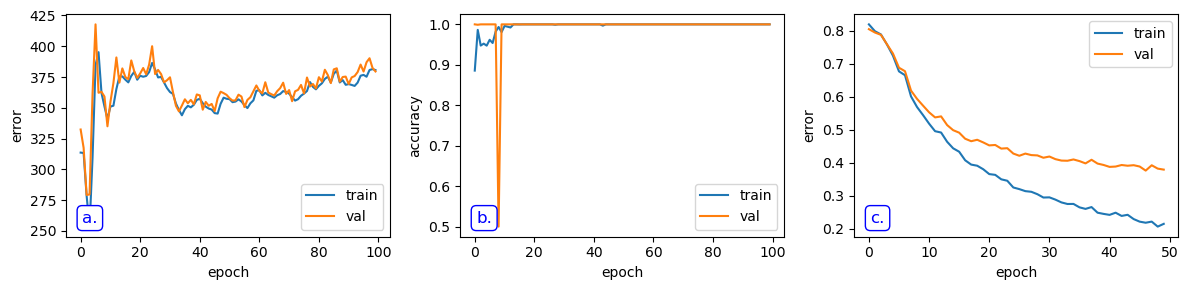
\includegraphics[width=\textwidth]{Figs/training-graphs.png}
    \end{center}
    \caption{Training and validation error / accuracy graphs during training process of each network. \textbf{a.} FID of the Generator. \textbf{b.} Accuracy of the Discriminator. \textbf{c.} CER of the Recognizer.}
    \label{fig:training_graphs}
\end{figure}

For comparison, our baseline Generator has FID of \textbf{273.9} on the images they generated, and the baseline Recognizer error rate of \textbf{0.4887}.

\section{Qualitative Results}
To show Generator qualitative results, we randomly selected 3 images generated by the best chosen model with input text from all validation samples. This is a straightforward way to directly show if the model is producing images we expect, and why the model is having an FID of \textbf{347.1}.

For the Recognizer, we selected the same 3 data as the ones we used for Generator qualitative results. The only difference is that we use the image validation samples instead of text validation samples. This helps conceptualize the quantitative CER of the model and how ``close'' it is reading from the texts.

Qualitative results from both networks are shown in Figure \ref{fig:valid_qualitative}.

\begin{figure}[!hbpt]
    \begin{center}
        \includesvg[width=\textwidth]{Figs/generator_recognizer_qual_val.svg}
    \end{center}
    \caption{Qualitative results of the final network using validation data. Top row consists the text input to the Generator as title and generated image from the Generator. Bottom row consists recognized text content from the Recognizer as title, input image, with CER below the input image.}
    \label{fig:valid_qualitative}
\end{figure}

The baseline model's qualitative results are shown in Figure \ref{fig:baseline_qualitative}, showing the baseline's output on the same input data for comparison.

\section{Evaluate Model on New Data}
To demonstrate the model's performance on never-seen-before data, we sampled texts from Shakespeare, which the model has never seen since the IAM database contains British texts produced in 1961 \citep{Marti1999AFE} \citep{corpus}. We input the text into Encoder and Generator, while we evaluate the Recognizer by using images of our team member's own handwriting of the Shakespeare texts, which went through similar pre-processing as the dataset used before.

The result of passing new data through the network yielded Generator FID \textbf{347.8} and Recognizer error \textbf{0.3968}. Randomly selected generated images and text recognition are shown in Figure \ref{fig:test_qualitative}.

\begin{figure}[!hbpt]
    \begin{center}
        \includesvg[width=\textwidth]{Figs/generator_recognizer_qual_test.svg}
    \end{center}
    \caption{Qualitative results of the final networks on Shakespeare texts. Top row consists the text input to the Generator as title and generated image from the Generator. Bottom row consists recognized text content from the Recognizer as title, input image, with CER below the input image.}
    \label{fig:test_qualitative}
\end{figure}

\section{Discussion}
\label{sec:discussion}
The validation Generator FID of \textbf{347.1} shows that the Generator model is performing poorly. Generally, an FID of higher than 200 indicates that the generated images have significant distortion and that they are very far from the expected ``real'' images. Since our model's validation FID is \textbf{347.1}, it shows that the generated images are not close to what we want the Generator to produce. The testing FID is \textbf{347.8}, which is only slightly higher than the validation FID, showing that the model is not overfitting, but very likely underfitting.

Looking at the qualitative results produced by the model for validation and testing from Figures \ref{fig:valid_qualitative} and \ref{fig:test_qualitative}, we can see visual confirmations that the Generator does not produce recognizable texts, which explains the high Generator FID. Furthermore, since FID compares the feature distribution of images, the fact that all the produced images look virtually identical regardless of input prompt can further contribute to the high FID score, since FID values diversity in the sample images.

Comparing our Generator's results with the baseline Generator shows that our Generator is under-performing compared to baseline. This can be seen through the baseline FID of \textbf{273.9} being significantly lower than our Generator's FID of \textbf{347.1}. Qualitative results also supports this since, even though images produced by the baseline generator has repeated characters, it is clearly legible and will not be seen as a computer-generated image at first glance.

It is interesting to note that the model output, despite not containing fully legible characters, forms some uniformly distributed black ``blobs'' or partial strokes at locations where characters commonly appears. This could be an indication that the model is only memorizing some features of characters, but not capable of replicating legible texts. A possible reason could be that these black ``blobs'' are where the ``average'' characters appears so the Generator was producing them as an attempt to ``trick'' the Discriminator. Another interesting phenomenon to discuss is the identical-looking generated images. This could indicate that the Generator does not allow the ``condition'' tensors (that is the noise and text embedding) to influence the model output sufficiently.

A potential reason for the Generator to not perform well is the fact that the Discriminator, despite having its learning rate tuned down, is still ``overpowering'' the Generator network. This can be seen from the discriminator accuracy graph in Figure \ref{fig:training_graphs}b, where the discriminator quickly reaches an accuracy of 1.0 and never goes down from there. When this happens, it is possible that the Discriminator captures features that benefits it, but in consequence causes these features, useless for the Generator, to be backpropagated anyway. This could lead the Generator to try converging in an non-ideal manner. We have noticed this during training, where the image background in generated images are turning more and more grey, causing less distinct textual features and lead to the rising FID for Generator as can be seen in Figure \ref{fig:training_graphs}a.

For the Recognizer, the validation CER of \textbf{0.3763} shows that only 37.63\% of the characters are predicted incorrectly, indicating that the Recognizer is correct on most portions of the input. Furthermore, our Recognizer model had a CER of \textbf{0.3968} on images it has never seen before, with both the content (the model has never read Shakespeare texts) and writing styles (the model has never been trained on our group member's handwriting before) being brand-new to the network. Even though the test error is slightly higher than the validation error, it is to be expected since the model was never tuned for this data, and the fact that the model is still capable of recognizing most of the input image's texts shows that the model is capable of generalizing. When compared to the baseline Recognizer error of \textbf{0.4887}, we can see that our model outperforms the baseline.

Reading what our model is outputting for validation, we can see that the CER of \textbf{0.3763} for validation slightly understates the accuracy of the network. We can see that sometimes the model predicts characters correctly, but they are shifted by one space, or that sometimes the model predicts individual characters incorrectly but instead predicts some characters extremely close to the expected character. In Figure \ref{fig:valid_qualitative}, the Recognizer predicted ``rougull--billl'' while the real text was ``roughly-built'', which is extremely close, but the CER would still increase the error rate as if it predicted some completely irrelevant text. Looking at the test qualitative results in Figure \ref{fig:test_qualitative}, we notice another phenomenon that the model seems to be recognizing mostly the earlier portion of the text correctly, while failing to recognize later portions of the text. This could be due to the fact that our data set always contains characters in the earlier portions of the text, but not all data contains text in the later parts of the text, causing the network to not be ``trained enough'' for longer texts. This is supported by our line dataset having a mean label length of \textbf{41.2} characters with standard deviation of \textbf{10.8} characters. One more interesting result of the Recognizer worth discussing is that in the test qualitative results in Figure \ref{fig:test_qualitative}, there are a lot of repeated characters being predicted. One possible reason is that the image dataset has writing styles with various sizes, so the model might be attempting to decode multiple characters from the same pixel groups, causing the same character to be repeatedly recognized.

Overall, we found this project to be quite challenging, and more difficult than expected. One of the main challenges was the sheer size of the GAN and the difficulties of tuning the hyperparameters to balance all three of the main sub-networks. While the generator, discriminator, and recognizer architectures were all functional on their own, balancing the discriminator and recognizer to produce a useful loss function and selecting the right learning rates proved to be extremely difficult. Since the network is so sensitive to the these hyperparameters, it was very challenging to tune each sub-network to make them compatible with each other. The size also made the network very time-consuming to train - even using features such as CUDA, the full GAN often took tens of hours to train, which limited the range of hyperparameters we were able to try.

Despite these challenges, we were able to produce a working model for each sub-network, and our recognizer outperforms the Pytesseract baseline model.

\section{Ethical Considerations}
Some ethical issues that may arise from the use of this model includes:

{\bf Forgery:} People could be using a handwriting synthesis model to replicate handwriting contents of others and fake documents (signatures, letters, journals, etc.). Even though the current model does not produce perfect images, it is still a possibility with an improved model.

    {\bf Representation Bias:} The training data presents ethical concerns, as the data we used (IAM dataset) contains only British texts in 1961, which may not accurately represent the vast diversity of what people write around the world. Furthermore, the data is handwritten by a few select individuals, likely not originated from diverse cultural / educational backgrounds, meaning the model may fail to produce / recognize the diversity of handwriting styles of all populations. It is essential to recognize the potential bias originating from the training data.

    {\bf Privacy Concerns:} When training the model to produce or to recognize handwriting images, the model ``memorizes'' the input training data. Which could potentially lead to the model ``leaking'' characteristics of the providers of the handwritings, such as their mental health, physical strength, education level, etc. Which could be possible to decode by some other tools. Also, there is another possibility of the model outputting near-exact content of the training data, hence leaking the original handwriting / text contents used to train the model.

\label{last_page}
\clearpage

\bibliography{ref}
\bibliographystyle{iclr2022_conference}

\end{document}
